\section{Four NP-Complete PMU Placement Problems}
\label{sec:problem-analysis}


In this section we define four PMU placement problems (\fulls, \maxincs, \xvals, and \xvalparts) and prove their NP-Completeness. 
\xval and \xvalpart both consider measurement error detection, while \full and \maxinc do not.  
We begin with a general overview of NP-Completeness, as well as a high-level description of the proof strategy used in this chapter (Section \ref{subsec:proofstrat}). 
In the remainder of Section \ref{sec:problem-analysis} we present and prove the NP-Completeness of four PMU placement problems, 
in the following order: \full (Section \ref{subsec:full}), \maxinc (Section \ref{subsec:maxinc}), \xval (Section \ref{subsec:xval}), and \xvalpart (Section \ref{subsec:xvalpart}).

In all four problems we are only concerned with computing the voltage phasors of each bus (i.e., observing the buses). Using the values of the voltage phasors,
Ohm's Law can be easily applied to compute the current phasors of each transmission line.
Also, we consider networks with both injection and zero-injection buses. For similar proofs for purely zero-injection systems, see Appendix \ref{ch:appendix-pmu}.


\subsection{NP-Completeness Overview and Proof Strategy}
\label{subsec:proofstrat}

Before proving that our PMU placement problems are NP-Complete (abbreviated NPC), we provide some background on NP-Completeness. 
NPC problems are the hardest problems in complexity class $\mathcal{NP}$. 
It is generally assumed that solving NPC problems is hard, meaning that any algorithm that solves an NPC problem has exponential running time as function of the input size. 
It is important to clarify that despite being NPC, a {\em specific} problem instance might be efficiently solvable. This is either due to the special structure of the specific instance 
or because the input size is small, yielding a small exponent. 
For example, in Section \ref{sec:simulations} we are able to solve \full for small IEEE bus topologies due to their small size. Thus, by establishing that our PMU placement problems are NPC, 
we claim that there {\em exist} bus topologies for which these problems are difficult to solve (i.e., no known polynomial-time algorithm exists to solve those case).  

To prove our problems are NPC, we follow the standard three-step reduction procedure. For a decision problem $\Pi$, we first show $\Pi\in\mathcal{NP}$. 
Second, we select a known NPC problem, denoted $\Pi'$, and construct a polynomial-time transformation, $f$, that maps any instance of $\Pi'$  to an instance of $\Pi$. 
Finally, we must ensure that for this $f$,  $x\in\Pi'\Leftrightarrow f(x)\in\Pi$ \cite{Garey79}.

Next, we outline the proof strategy we use throughout this section. In Sections  \ref{subsec:full} through Section \ref{subsec:xvalpart} we use slight variations of the approach presented
by Brueni and Heath in \cite{Brueni05} to prove the problems we consider here are NPC. In general we found their scheme to be elegantly extensible for proving many properties of PMU placements.

In \cite{Brueni05}, the authors prove NP-Completeness by reduction from planar 3-SAT (\sats). A 3-SAT formula, $\phi$, is a boolean formula in conjunctive normal form (CNF) such that each clause contains at most $3$ literals. For any 3-SAT formula $\phi$ with the sets of variables $\{v_1,v_2, \dots , v_r\}$ and clauses $\{c_1,c_2, \dots , c_s \}$, $G(\phi)$ is the bipartite graph $G(\phi)=(V(\phi),E(\phi))$ defined as follows:
\begin{eqnarray*}
 V(\phi) &= &\{v_i\; \vert\; 1 \leq i \leq r \} \cup \{c_j \;\vert\; 1 \leq j \leq s \} \\
 E(\phi) &=& \{ (v_i,c_j)\;\vert\; v_i \in c_j\;\; or \;\; \overline{v_i} \in c_j\}.
\end{eqnarray*}
Note that edges pass only between $v_i$ and $c_j$ nodes, and so the graph is bipartite.  \sat is a 3-SAT formula such that $G(\phi)$ is planar \cite{Lich82}. 
For example, \sat formula
\begin{eqnarray}
\varphi  &=& (\overline{v_1} \vee v_2 \vee v_3) \wedge (\overline{v_1} \vee \overline{v_4} \vee v_5) \wedge (\overline{v_2} \vee \overline{v_3} \vee \overline{v_5}) \nonumber\\
		 & & \wedge (v_3 \vee \overline{v_4}) \wedge  (\overline{v_3} \vee v_4 \vee \overline{v_5})
\label{eqn:varphi}
\end{eqnarray}
has graph $G(\varphi)$ shown in Figure \ref{fig:gvarphi}. Discovering a satisfying assignment for  \sat is an NPC problem, and so it can be used in a reduction to prove the complexity of the problems we address here. Note that in this work we will use $\varphi$ to denote a specific \sat formula, while $\phi$ will be used to denote a generic \sat formula.

Following the approach in \cite{Brueni05}, for \sat formula, $\phi$, we replace each variable node and each clause node in $G(\phi)$ with a specially constructed set of nodes,
termed a {\em gadget}. In this work, all variable gadgets will have the same structure, and all clause gadgets have the same structure (that is different from the variable gadget structure), 
and we denote the resulting graph as $H(\phi)$. In $H(\phi)$, each {\em variable} gadget has a subset of nodes that semantically represent assigning ``True" to that variable, and a subset of 
nodes that represent assigning it ``False". When a PMU is placed at one of these nodes, this is interpreted as assigning a truth value to the \sat variable corresponding with that gadget. 
Thus, we use the PMU placement to determine a consistent truth value for each \sat variable. Also, clause gadgets are connected to variable gadgets at either ``True" or ``False" (but never both) 
nodes, in such a way that the clause is satisfied if and only if {\em at least one} of those nodes has a PMU.

Although the structure of our proofs is adapted from \cite{Brueni05}, the variable and clause gadgets we use to correspond to the \sat formula are novel, thus leading to a 
different set of proofs. Our work here demonstrates how the approach from \cite{Brueni05} can be extended, using new variable and clause gadgets, to address a wide array of PMU placement problems.

While we assume $G(\phi)$ is planar, we make no such claim regarding $H(\phi)$, though in practice all graphs used in our proofs are indeed planar. The proof of NPC rests on the fact that 
solving the underlying $\phi$ formula is NPC. In what follows, for a given PMU placement problem $\Pi$, we prove $\Pi$ is NPC by showing that a PMU placement in $H(\phi)$, $\Phi$, can be 
interpreted semantically as describing a satisfying assignment for $\phi$ iff $\Phi\in\Pi$. 
Since \sat is NPC, this proves $\Pi$ is  NPC as well. 



\begin{figure}

\subfigure[$G(\varphi)$ formed from $\varphi$ in Equation (\ref{eqn:varphi}).]{\label{fig:gvarphi}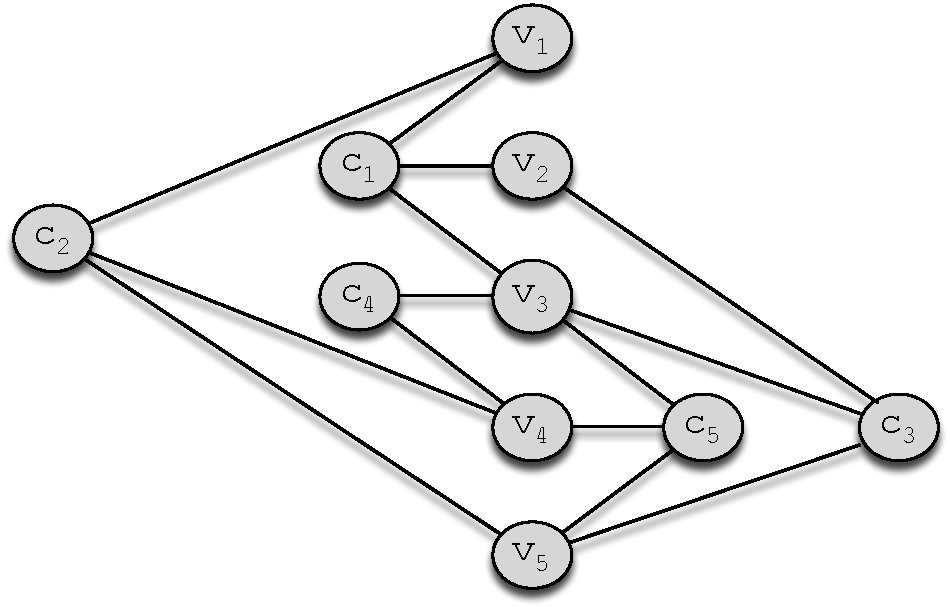
\includegraphics[scale=0.53]{figs/gvarphi.pdf}}
\subfigure[Graph formed from $\varphi$ formula in Theorem \ref{thm:npc-full} proof.] %Nodes with a dashed border are zero-injection nodes.]
{\label{fig:gvarphi2}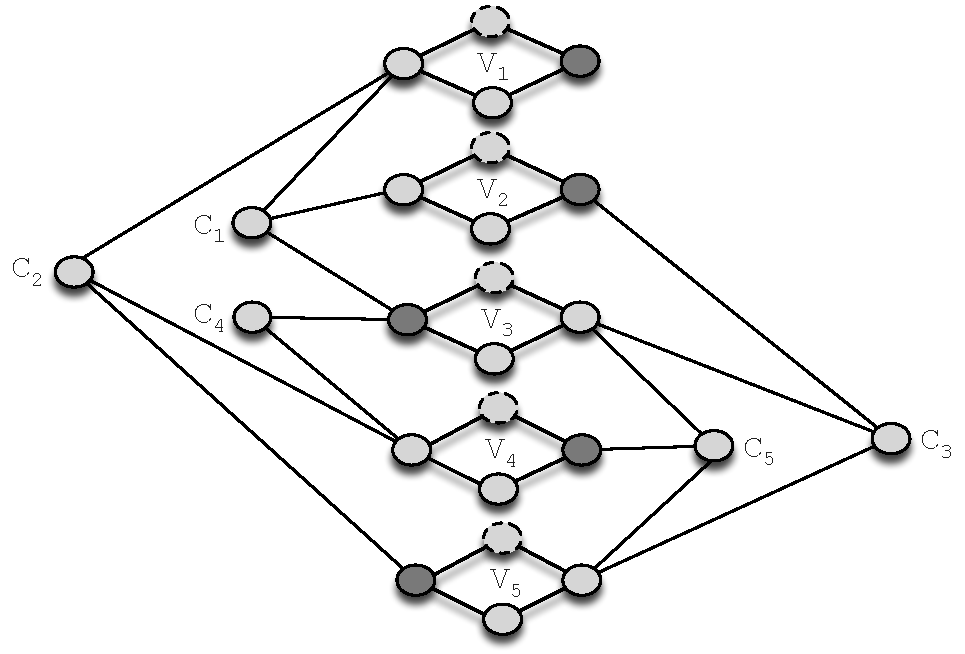
\includegraphics[scale=0.53]{figs/proof1-inject-example.pdf}}

\caption{The figure in (a) shows $G(\varphi)=(V(\varphi),E(\varphi))$ using example formula, $\varphi$, from Equation (\ref{eqn:varphi}).  (b) shows the new graph formed by replacing each variable
node in $G(\varphi)$ -- as specified by the Theorem \ref{thm:npc-full} proof -- with the Figure \ref{fig:diamond-gadget} variable gadget. 
%using the variable clause in Figure \ref{fig:diamond-gadget} and a single clause node.
} 
\end{figure}




\begin{figure}
    \fbox{\subfigure[Variable gadget used in Theorem \ref{thm:npc-full} and \ref{thm:npc-maxinc}.]
	{\label{fig:diamond-gadget}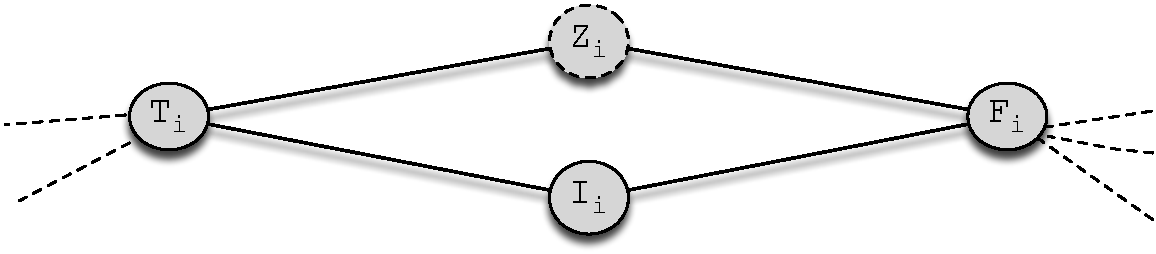
\includegraphics[scale=0.31]{figs/diamond-gadget.pdf}}}
	\fbox{\subfigure[Theorem \ref{thm:npc-maxinc} clause gadget.]
	{\label{fig:line-gadget}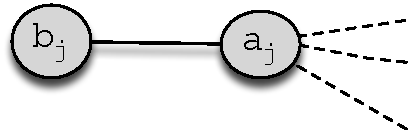
\includegraphics[scale=0.31]{figs/line-gadget.pdf}}}
	\fbox{\subfigure[Variable gadget used in Theorem \ref{thm:npc-xval}, containing two disconnected subgraphs.]
	{\label{fig:xval-gadget}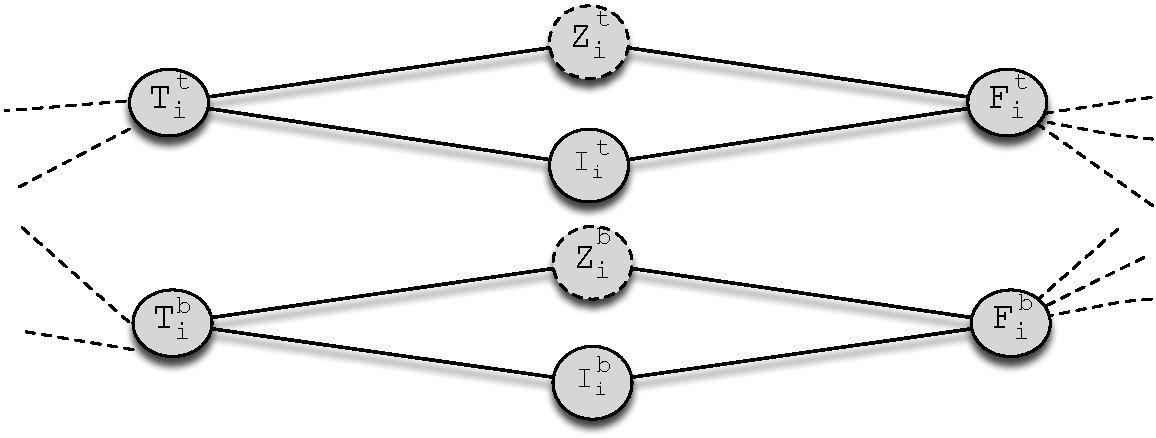
\includegraphics[scale=0.31]{figs/vgadget-inject.pdf}}}

	\caption{Gadgets used in Theorem \ref{thm:npc-full} - \ref{thm:npc-xvalpart}. $Z_i$ in Figure \ref{fig:diamond-gadget}, $Z_i^t$ in Figure \ref{fig:xval-gadget}, and $Z_i^b$ in Figure \ref{fig:xval-gadget} are the only zero-injection nodes.
	The dashed edges in Figure \ref{fig:diamond-gadget} and Figure \ref{fig:xval-gadget} are connections to clause gadgets. Likewise, the dashed edges in Figure (b) are connections to variable gadgets.  In Figure \ref{fig:xval-gadget},
	superscript, $t$, denotes nodes in the upper subgraph and superscript, $b$, indexes nodes in the lower subgraph.}
	%\caption{Graph $G=(V,E)=H_1(\varphi)$ formed from $\varphi$ formula in Theorem \ref{thm:npc-full} proof. Nodes with a dashed border are zero-injection nodes.}
  
\label{fig:pmu-gadgets}
\end{figure}


\subsection{The \full Problem}
\label{subsec:full}

The \full problem has been addressed in the literature (e.g., the PMUP problem in \cite{Brueni05}, and the PDS problem in \cite{Haynes02}) but only for purely zero-injection bus systems. 
Here we consider networks with mixtures of injection and zero-injection buses, and modify the NPC proof of PMUP in \cite{Brueni05} to handle this mixture.
\\
{\bf \full Optimization Problem:}\\
\indent \underline{Input}: Graph $G=(V,E)$ where $V=V_Z \cup V_I$ and $V_Z \neq \emptyset$.
	{\footnote {\small We include the condition that $V_Z \neq \emptyset$ because otherwise \full reduces to \textsc{Vertex-Cover}, making the NP-Completeness
	proof trivial.}} \\
\indent \underline{Output}: A placement of PMUs, $\Phi_G$, such that $\Phi^R_G=V$ and $\Phi_G$ is minimal.
\\
{\bf \full Decision Problem:} \\
\indent \underline{Instance}: Graph $G=(V,E)$ where $V=V_Z \cup V_I$, $V_Z \neq \emptyset$, $k$ PMUs such that $k \geq 1$. \\
\indent \underline{Question}: Is there a $\Phi_G$ such that $|\Phi_G| \leq k$ and $\Phi^R_G = V$?


\begin{theorem}
\full is NP-Complete. %even when restricted to the class of bipartite planar graphs.
\label{thm:npc-full}
\end{theorem}

{\bf Proof Idea}:  We introduce a problem-specific variable gadget. We show that in order to observe all nodes, PMUs must be placed on variable gadgets, specifically on
nodes that semantically correspond to True and False values that satisfy the corresponding \sat formula. 

For our first problem, we use a single node as a clause gadget denoted $a_j$, and the subgraph shown in Figure \ref{fig:diamond-gadget} as the variable gadget. Note that in the variable gadget, all the nodes are injection nodes except for $Z_i$. For this subgraph, we state the following simple lemma:

\begin{lemma}\label{lem:property1}
Consider the gadget shown in Figure \ref{fig:diamond-gadget}, possibly with additional edges connected to $T_i$ and/or $F_i$. Then (a) nodes $I_i, Z_i$ are not observed if there is no PMU on the gadget, and (b) all the nodes in the gadget are observed with a single PMU iff the PMU is placed on either $T_i$ or $F_i$.
\end{lemma}
\begin{proof}
(a) If there is no PMU on the gadget, O1 cannot be applied at any of the nodes, and so we must resort to O2. We assume no edges connected to $I_i,Z_i$ from outside the gadget, and since $T_i,F_i\in V_I$, we cannot apply O2 at them, which concludes our proof.
 
(b) In one direction, if we have a PMU placed at $T_i$, from O1 we can observe $Z_i,I_i$. Since $Z_i$ is zero-injection and one neighbor, $T_i$ has been observed, from O2 at $Z_i$ we can observe $F_i$. The same holds for placing a PMU at $F_i$, due to symmetry.

In the other direction, by placing a PMU at $I_i$ ($Z_i$) we observe $T_i$ and $F_i$ via O1. However, since $F_i,T_i\notin V_Z$, O2 cannot be applied at either of them, so $Z_i$ ($I_i$) will not be observed. 
\end{proof}

\begin{proof}[Proof of Theorem \ref{thm:npc-full}]
%\begin{proof}
%\maxinc is easily in $\in \mathcal{NP}$.
We start by arguing that \full $\in \mathcal{NP}$. First, nondeterministically select $k$ nodes in which to place PMUs. Using the rules specified in Section \ref{subsec:observe}, determining
the number of observed nodes can be done in linear time.
%Haynes et al. \cite{Haynes02} show that given a PDS solution can be verified in polynomial time. Since \maxinc only checks $m < |V|$ vertices,
%the same algorithm can be used to verify a \maxinc solution in polynomial time.

To show \full is NP-hard, we reduce from \sats.  Let $\phi$ be an arbitrary \sat formula with variables 
$\{v_1,v_2, \dots , v_r\}$ and the set of clauses $\{c_1,c_2,\dots , c_s \}$, and $G(\phi)$ the corresponding planar graph. We use $G(\phi)$ to construct a new graph $H_0(\phi) = (V_0(\phi), E_0(\phi))$ by replacing each variable
node in $G(\phi)$ with the variable gadget shown in Figure \ref{fig:diamond-gadget}. The clause nodes consist of a single node (i.e., are the same
as in $G(\phi)$). We denote the node corresponding to $c_j$ as $a_j$. All clause nodes are injection nodes.  In the remainder of this proof we let $H := H_0(\phi)$.
In total, $V_Z$ contains all $Z_i$ nodes for $1 \leq i \leq r$, and all other nodes are in $V_I$.  The edges connecting clause nodes with variable gadgets express which variables are in each clause: for each clause node $a_j$, $(T_i, a_j)\in E_0(\phi) \Leftrightarrow v_i\in c_j$, and $(F_i, a_j)\in E_0(\phi) \Leftrightarrow \overline{v_i}\in c_j$. As a result, the following observation holds:

\begin{observation}\label{obs:1}
For a given truth assignment and a corresponding PMU placement, a clause $c_j$ is satisfied iff $a_j$ is attached to a node in a variable gadget with a PMU. 
\end{observation}


The resulting graph for the example given in Figure \ref{fig:gvarphi} is shown in Figure \ref{fig:proof1-inject-example}.  Nodes with a dashed border are zero-injection nodes. 
{\footnote {\small  Throughout this chaper, nodes with dashed borders denote zero-injection nodes. }} 
The corresponding formula for this graph, $\varphi$,
is satisfied by truth assignment $A_{\varphi}$: $\overline{v_1}, \overline{v_2}, v_3, \overline{v_4},$ and $\overline{v_5}$ are True. This corresponds to the dark shaded nodes in Figure
\ref{fig:gvarphi2}. While this construction generates a graph with very specific structure, in Section \ref{subsec:extend}, we detail how to extend our proof to consider graphs with a wider range of structures.% different $\frac{|V_Z|}{|V_I|}$ ratios.


With this construct in place, we move on to our proof. We show that $\phi$ is satisfiable if and only if $k=r=|\Phi_H|$ PMUs
can be placed on $H$ such that $\Phi^R_{H}=V$.

$(\Rightarrow)$ Assume $\phi$ is satisfiable by truth assignment $A_{\phi}$. Then, consider the placement $\Phi_H$ such that for each variable gadget $V_i$, $T_i\in \Phi_H \Leftrightarrow v_i=True$
in $A_\phi$, and  $F_i\in \Phi_H \Leftrightarrow v_i=False$. From Lemma \ref{lem:property1}(b) we know that all nodes in variable gadgets are observed by such a placement. From Observation \ref{obs:1}, all clause nodes are observed because our PMU assignment is based on a satisfying assignment.
Thus, we have shown that $\Phi^R_{H}=V$.

$(\Leftarrow)$
Suppose there is a placement of $r$ PMUs, $\Phi_H$, such that $\Phi_H^R = V$.  From Lemma \ref{lem:property1}(a) we know that for each $V_i$ with no PMU, at least two nodes are not observed, so each $V_i$  must have a PMU placed in it. 
Since we have only $r$ PMUs, that means one PMU per gadget. From Lemma \ref{lem:property1}(b) we know this PMU must be placed on $T_i$ or $F_i$, since otherwise the gadget will not be fully observed. Note that these nodes are all in $V_I$.

Since we assume the graph is fully observed, all $a_j$ are observed by $\Phi_H$. Because we just concluded that PMUs are placed only on injection nodes in the variable gadgets, each clause node $a_j$ can only be observed via application of O1 at $T_i/F_i$ nodes to which it is attached -- specifically, $a_j$ is attached to a node with a PMU. From Observation \ref{obs:1} this means that all clauses are satisfied by the semantic interpretation of our PMU placement, which concludes our proof. 
\end{proof}

\subsection{The \maxinc Problem}
\label{subsec:maxinc}

\maxinc is a variation of \fulls: rather than consider the minimum number of PMUs required for full system observability,
\maxinc finds the maximum number of nodes that can be observed using a fixed number of PMUs.
\\
{\bf \maxinc Optimization Problem:} \\
	\indent \underline{Input}: Graph $G=(V,E)$ where $V=V_Z \cup V_I$, $k$ PMUs such that $1 \leq k < k^*$. \\
	\indent \underline{Output}: A placement of $k$ PMUs, $\Phi_G$, such that $|\Phi^R_G|$ is maximum. 
\\
{\bf \maxinc Decision Problem:} \\
	\indent \underline{Instance}: Graph $G=(V,E)$ where $V=V_Z \cup V_I$, $k$ PMUs such that $1 \leq k < k^*$.	 \\
	\indent \underline{Question}: For a given $m< |V|$, is there a $\Phi_G$ such that $|\Phi_G| \leq k$ and $m \leq |\Phi^R_G| < |V|$?


\begin{theorem}
\maxinc is NP-Complete. %even when restricted to the class of bipartite planar graphs.
\label{thm:npc-maxinc}
\end{theorem}

{\bf Proof Idea}: First, we construct problem-specific gadgets for variables and clauses. We then demonstrate that any solution that observes $m$ nodes must place the PMUs only on nodes
in the variable gadgets. Next we show that as a result of this, the problem of observing $m$ nodes in this graph reduces to Theorem \ref{thm:npc-full}.

\begin{proof}
%\maxinc is easily in $\in \mathcal{NP}$.
\maxinc $\in \mathcal{NP}$ using the same argument in the proof for Theorem \ref{thm:npc-full}.

Next, we reduce from {\sat} as in the proof for Theorem \ref{thm:npc-full}, where $\phi$ is an arbitrary \sat formula. We create a new graph $H_1(\phi) = (V_1(\phi), E_1(\phi))$ which is identical to $H_0(\phi)$ from the previous proof, except that each clause node in $H_0(\phi)$ is replaced with the clause gadget shown in Figure \ref{fig:line-gadget}, comprising of two injection nodes. As before, the edges connecting clause nodes with variable gadgets express which variables are in each clause: for each clause node $a_j$, $(T_i, a_j)\in E_1(\phi) \Leftrightarrow v_i\in c_j$, and $(F_i, a_j)\in E_1(\phi) \Leftrightarrow \overline{v_i}\in c_j$. Note that Observation \ref{obs:1} holds here as well.




We are now ready to show \maxinc is NP-hard. For convenience, we let $H := H_1(\phi)$.  Recall $\phi$ has $r$ variables and $s$ clauses. 
Here we consider the instance of \maxinc where $k=r$ and $m = 4r + s$, and show that $\phi$ is satisfiable if and only if $r=|\Phi_H|$ PMUs
can be placed on $H$ such that $m \leq |\Phi^R_{H}| < |V|$. In Section \ref{subsec:extend} we discuss how to extend this proof for any larger value of $m$ and different $\frac{|V_Z|}{|V_I|}$ ratios.

$(\Rightarrow)$ Assume $\phi$ is satisfiable by truth assignment $A_{\phi}$. Then, consider the placement $\Phi_H$ such that for each variable gadget $V_i$, $T_i\in \Phi_H \Leftrightarrow v_i=True$
in $A_\phi$, and  $F_i\in \Phi_H \Leftrightarrow v_i=False$.  In the proof for Theorem \ref{thm:npc-full} we demonstrated such a placement will observe all nodes in $H_0(\phi)\subset H_1(\phi)$, and using the same argument it can easily be checked that these nodes are still observed in $H_1(\phi)$. Each $b_j$ node remains unobserved because each $a_j \in V_I$ and consequently O2 cannot be applied at $a_j$.
Since $|H_0(\phi)|=4r+s = m$, we have observed the required nodes.

$(\Leftarrow)$
We begin by proving that any solution that observes $m$ nodes must place the PMUs only on nodes in the variable gadgets. By construction, each PMU is either on a clause gadget or a variable gadget, but not both. Let $0\leq t\leq r$ be the number of PMUs on clause gadgets, we wish to show that for the given placement $t=0$. First, note that {\em at least} $\max(s-t,0)$ clause gadgets are without PMUs, and that for each such clause (by construction) at least one node ($b_i$) is not observed. Next, from Lemma \ref{lem:property1}(a) we know that for each variable gadget without a PMU, at least two nodes are not observed.

Denote the {\em unobserved} nodes for a given PMU placement as $\Phi_H^-$. Thus, we get $|\Phi_H^-| \geq 2t + \max((s-t), 0)$. However, since $m$ nodes are observed and  $|V|-m \leq s$, we get $|\Phi_H^-| \leq s$, so we know $s \geq 2t + \max((s-t), 0)$. We consider two cases:
\begin{itemize}
	\item $s\geq t$: then we get $s \geq t + s \Rightarrow t=0.$
	\item $s < t$:	then we get $s \geq 2t$, and since we assume here $0\leq s < t$ this leads to a contradiction and so this case cannot occur.
\end{itemize}

Thus, the $r$ PMUs must be on nodes in variable gadgets. Note that the variable gadgets in $H_1(\phi)$ have the same structure as in $H_0(\phi)$. We return to this point shortly.

Earlier we noted that for each clause gadget without a PMU, the corresponding $b_j$ node is unobserved, which comes to $s$ nodes. To observe $m=4r+s$ nodes, we will need to observe all the remaining nodes. Thus, we have reduced the problem to that of observing all of $H_0(\phi)\subset H_1(\phi)$. Our proof for Theorem \ref{thm:npc-full} demonstrated this can only be done by placing PMUs at nodes corresponding to a satisfying assignment of $\phi$, and so our proof is complete. 
\end{proof}


\subsection{The \xval Problem}
\label{subsec:xval}

The \xval optimization and decision problems are defined as follows:
\\
{\bf \xval Optimization Problem:} \\
	\indent \underline{Input}: Graph $G=(V,E)$ where $V=V_Z \cup V_I$. \\
	\indent \underline{Output}: A placement of PMUs, $\Phi_G$, such that $\Phi^R_G = V$,
	and  $\Phi_G$ is minimal under the condition that each $v \in \Phi_G$ is cross-validated according to the rules specified in Section \ref{subsec:xval-rules}.
\\
{\bf \xval Decision Problem:} \\
	\indent \underline{Instance}: Graph $G=(V,E)$ where $V=V_Z \cup V_I$, $k$ PMUs such that $k \geq 1$. \\
	\indent \underline{Question}: Is there a $\Phi_G$ such that $|\Phi_G| \leq k$ and $\Phi^R_G = V$ under the condition that each $v \in \Phi_G$ is cross-validated?



\begin{theorem}
\xval is NP-Complete. % even when restricted to the class of bipartite and chordal graphs.
\label{thm:npc-xval}
\end{theorem}



{\bf Proof Idea:}   We show \xval is NP-hard by reducing from \sats.  
We create a single-node gadget for clauses (as for \fulls) and the gadget shown in Figure \ref{fig:xval-gadget} for each variable. Each variable gadget here comprises of two disconnected components, 
and there are two $T_i$ and two $F_i$ nodes, one in each component. First, we show that each variable gadget must have $2$ PMUs for the entire graph to be observed, one PMU for each subgraph.
Then, we show that cross-validation constraints force PMUs to be placed on both $T$ nodes or both $F$ nodes.  Finally, we show how to use the PMU placement to derive a satisfying \sat truth assignment.
 
%Our proof makes use of the following Lemma.  Note that for each variable gadget $V_i$, we refer to the upper subgraph as $V_{i}^t$ and the
%lower subgraph as $V_{i}^b$.

\begin{lemma}\label{lem:property2}
Consider the gadget shown in Figure \ref{fig:xval-gadget}, possibly with additional nodes attached to $T_i$ and/or $F_i$ nodes. (a) nodes $I^t_i, Z^t_i$ are not observed if there is no PMU on $V_i^t$, and (b) all the nodes in $V_i^t$ are observed with a single PMU iff the PMU is placed on either $T_i^t$ or $F_i^t$. Due to symmetry, the same holds when considering $V_i^b$.
\end{lemma}
\begin{proof}
The proof is straightforward from the proof of Lemma \ref{lem:property1}, since both $V_i^t$ and $V_i^b$ are identical to the gadget from Figure \ref{fig:diamond-gadget},  which Lemma \ref{lem:property1} refers to. 
\end{proof}

\begin{proof}[Proof of Theorem \ref{thm:npc-xval}]
First, we argue that \xval $\in \mathcal{NP}$.  Given a \xval solution, we use
the polynomial time algorithm described in our proof for Theorem
\ref{thm:npc-full} to determine if all nodes are observed.  Then, for each
PMU node we run a breadth-first search, stopping at depth $2$, to check that
the cross-validation rules are satisfied.

To show \xval is NP-hard, we reduce from \sats.  Our reduction is similar to
the one used in Theorem \ref{thm:npc-full}.  We start with the same \sat formula $\phi$ with variables $\{v_1,v_2, \dots , v_r\}$ and the set of clauses $\{c_1,c_2,\dots , c_s \}$.

% Given a \sat formula, $\phi$,
% with variables $\{v_1,v_2, \dots , v_r\}$ and the set of clauses $\{c_1,c_2,
% \dots , c_s \}$, we form a new graph, $G=(V,E)$, as follows. Each clause $c_j$
% corresponds to a pair of nodes connected by an edge, denoted $C[j],C'[j]$. This
% is the same construct as described in the original proof \cite{Brueni05}.
For this problem, we construct $H_2(\phi)$ in the following manner. We use the single-node clause gadgets  as in $H_0(\phi)$, and as before, the edges connecting clause nodes with variable gadgets shown in Figure \ref{fig:xval-gadget} express which variables are in each clause: for each clause node $a_j$, $(T^t_i, a_j),(T^b_i, a_j)\in E_1(\phi) \Leftrightarrow v_i\in c_j$, and $(F^t_i, a_j),(F^b_i, a_j)\in E_1(\phi) \Leftrightarrow \overline{v_i}\in c_j$. For notational simplicity, we shall use $H$ to refer to $H_2(\phi)$. Note that once again, by construction Observation \ref{obs:1} holds for $H$.

%Let $k = 2r$.
Moving on, we now show that $\phi$ is satisfiable if and only if
$k=2r$ PMUs can be placed on $H$ such that $H$ is fully observed under the
condition that all PMUs are cross-validated, and that $2r$ PMUs are the minimal
bound for observing the graph with cross-validation.

$(\Rightarrow)$ Assume $\phi$ is satisfiable by truth assignment $A_{\phi}$.
For each $1\leq i\leq r$, if $v_i=True$ in $A_{\phi}$ we place a PMU at $T_i^b$
and at $T_i^t$ of the variable gadget $V_i$. Otherwise, we place a PMU at $F_i^b$
and at $F_i^t$ of this gadget. From the fact that $A_{\phi}$ is satisfying and Observation \ref{obs:1}, we know the PMU nodes in $V_i$ must be
adjacent to some clause node\footnote{Each variable must be used in at least a single clause, or it is not considered part of the formula. If there is a variable that has no impact on the truth value of $\phi$, we always place the PMUs on two nodes (both T or both F) that are adjacent to a clause node.}, making $T_i^t$ ($F_i^t$) two hops away from
$T_i^b$ ($F_i^b$). Therefore, all PMUs are cross-validated by XV2.

Assignment $\Phi_H$ observes all $v \in V$: from Lemma \ref{lem:property2}(b) we know the assignment fully observes all the variable gadgets. From Observation \ref{obs:1} we know all clause nodes are adjacent to a node with a PMU, so they are observed via O1, which concludes this direction of the theorem.

$(\Leftarrow)$ Suppose $\Phi_G$ observes all nodes in $H$
under the condition that each PMU is cross-validated, and that $|\Phi_H|=2r$. We want to show that
$\phi$ is satisfiable by the truth assignment derived from $\Phi_H$. We do so following a similar method as for the previous Theorems.

From Lemma \ref{lem:property2}(a) we know that each component in each variable gadget must have at least one PMU in order for the entire graph to be observed. Since we have $2r$ PMUs and $2r$ components, each component will have a single PMU. This also means there are no PMUs on clause gadgets.

From Lemma \ref{lem:property2}(b) we know that full observability will require PMUs  be on either $T$ or $F$ nodes in each variable gadget. As a result,  cross-validation constraints require for each variable gadget that both PMUs are either on $T_i^t, T_i^b$ or $F_i^t, F_i^b$. This is because any $T_i^t$ ($F_i^t$) is four hops or more away from any other $T/F$ node. Since we assume the clause nodes are all observed and we know no PMUs are on clause nodes, from Observation \ref{obs:1} this means the PMU placement satisfies all clauses, which concludes our proof.
\end{proof}



\subsection{The \xvalpart Problem}
\label{subsec:xvalpart}

The \xvalpart optimization and decision problems are defined below:
\\
{\bf \xvalpart Optimization Problem:} \\
	\indent \underline{Input}: Graph $G=(V,E)$ where $V=V_Z \cup V_I$ and $k$ PMUs such that $1 \leq k < k^*$. \\
	\indent \underline{Output}: A placement of $k$ PMUs, $\Phi_G$, such that $|\Phi^R_G|$ is maximum under the condition that
	each $v \in \Phi_G$ is cross-validated according to the rules specified in Section \ref{subsec:xval-rules}.
\\
{\bf \xvalpart Decision Problem:} \\
	\indent \underline{Instance}: Graph $G=(V,E)$ where $V=V_Z \cup V_I$, $k$ PMUs such that $1 \leq k < k^*$, and some $m<|V|$. \\
	\indent \underline{Question}: Is there a $\Phi_G$ such that $|\Phi_G| \leq k$ and $m \leq|\Phi^R_G| < |V|$ under the condition that each $v \in \Phi_G$ is cross-validated?

%The corresponding {\em optimization problem} is to find the maximal $m$ such that $m$ nodes can be observed using $k$ PMUs and while cross-validating all PMUs. A formal definition of the optimization problem 
%can be found in the technical report \xxx{CITE}. 


\begin{theorem}
\xvalpart is NP-Complete. % even when restricted to the class of bipartite and chordal graphs.
\label{thm:npc-xvalpart}
\end{theorem}

%{\bf Proof Idea:} We show \xvalpart is NP-hard by reducing from \sats. Our proof is a combination of the techniques introduced in the NP-hardness proofs for \maxinc and \xvals,
%and is presented here at a high-level only with the details left to the reader to verify.\\
%From a \sat formula, we create a graph $G$ with the clause gadgets from \maxinc (Figure \ref{fig:clause-gadget}) and the variable gadgets from \xval (Figure \ref{fig:xval-gadget}).
%The edges in $G$ connecting clause and variable gadgets are the same as in $H_2(\varphi)$, and consider a proof with $m = |V|-2s$ as with \maxinc.

{\bf Proof Idea:} We show \xvalpart is NP-hard by reducing from \sats. Our proof is a combination of the NP-hardness proofs for \maxinc and \xvals.
From a \sat formula, $\phi$, we create a graph $G=(V,E)$ with the clause gadgets from \maxinc (Figure \ref{fig:line-gadget}) and the variable gadgets from \xval (Figure \ref{fig:xval-gadget}).
The edges in $G$ are identical the ones the graph created in our reduction for \xvals.

We show that any solution that observes $m=|V|-s$ nodes must place the PMUs exclusively on nodes in the variable gadgets. As a result, we show
$1$ node in each clause gadget -- $b_j$ for clause $C_j$ -- is not observed, yielding a total $s$ unobserved nodes. This implies all other nodes must be
observed, and thus reduces our problem to the scenario considered in Theorem \ref{thm:npc-xval}, which is already proven.


\begin{proof}
\xvalpart is easily in $\mathcal{NP}$. We verify a \xvalpart solution using the same polynomial time algorithm described in our proof
for Theorem \ref{thm:npc-xval}. % used to verify an \xval solution.

We reduce from \sat to show \xvalpart is NP-hard. Our reduction is a combination
of the reductions used for \maxinc and \xvals. Given a \sat formula, $\phi$,
with variables $\{v_1,v_2, \dots , v_r\}$ and the set of clauses $\{c_1,c_2,
\dots , c_s \}$, we form a new graph, $H_3(\phi) = (V(\phi),E(\phi))$  as follows. Each clause $c_j$
corresponds to the clause gadget from \maxinc (Figure \ref{fig:line-gadget})
and the variable gadgets from \xval (Figure \ref{fig:xval-gadget}).
As in Theorem \ref{thm:npc-xval}, we refer to the upper subgraph of variable gadget, $V_i$,
as $V_{i}^t$ and the lower subgraph as $V_{i}^b$.  Also, we denote here $H:= H_3(\phi)$.

Let $k = 2r$ and $m = 8r + s = |V| - s$. As in our NP-hardness proof for \maxincs, $m$ includes all nodes in $H$
except $b_j$ of each clause gadget. We need to show that $\phi$ is satisfiable if and only if
$2r$ cross-validated PMUs can be placed on $H$ such that $m \leq |\Phi^R_{H}| < |V|$.

$(\Rightarrow)$ Assume $\phi$ is satisfiable by truth assignment $A_{\phi}$.
For each $1\leq i\leq r$, if $v_i=True$ in $A_{\phi}$ we place a PMU at $T_i^b$
and at $T_i^t$ of the variable gadget $V_i$. Otherwise, we place a PMU at $F_i^b$
and at $F_i^t$ of this gadget. In either case, the PMU nodes in $V_i$ must be
adjacent to a clause node, making $T_i^t$ ($F_i^t$) two hops away from
$T_i^b$ ($F_i^b$)\footnote{See previous note on \xval}. Therefore, all PMUs are cross-validated by XV2.

This placement of $2r$ PMUs, $\Phi_H$, is exactly the same one derived from $\phi$'s satisfying instance in Theorem \ref{thm:npc-xval}.
Since $\Phi_H$ only has PMUs on variable gadgets, all $a_j$ nodes are observed by the same argument used in Theorem \ref{thm:npc-xval}.
Thus, at least $8r + s$ nodes are observed in $H$.
Because no PMU in $\Phi_H$ is placed on a clause gadget, $C_j$, and O2 cannot be applied at $a_j$ since $a_j \in V_I$, we know that no $b_j$ is observed.
We conclude that exactly $m$ nodes are observed with $\Phi_H$.

$(\Leftarrow)$
We begin by proving that any solution that observes $m$ nodes must place the PMUs only on nodes in the variable gadgets. Assume that there are $1<t\leq r$ variable gadgets without a PMU.
Then, at most $t$ PMUs are on nodes in clause gadgets, so {\it at least} $\max(s-t,0)$ clause gadgets are without PMUs. We want to show here that for $m=8r+s$, $t=0$.

To prove this, we rely on the following observations:
\begin{itemize}
	\item As shown in Theorem \ref{thm:npc-xval}, a variable gadget's subgraph with no PMU has at least $2$ unobserved nodes.
	\item In any clause gadget $C_j$, $b_j$ nodes cannot be observed if there is no PMU somewhere in $C_j$.
\end{itemize}
Thus, given some $t$, $|\Phi_H^-| \geq 2t + \max(s-t, 0)$, where $\Phi_H^-$ denotes the unobserved nodes in $H$. Since $|V|-m \leq s$, we know $|\Phi_H^-|\leq s$ and thus 
$s \geq 2t + \max(s-t, 0)$. We consider two cases:
\begin{itemize}
	\item $s\geq t$: then we get $s \geq s+t \Rightarrow t=0.$
	\item $s < t$:	then we get $s \geq 2t$, and since we assume here $0\leq s < t$ this leads to a contradiction and so this case cannot occur.
\end{itemize}

Thus, we have concluded that the $2r$ PMUs must be on variable gadgets, leaving all clause gadgets without PMUs. %, which, it is important to note, were also part of the original $H(\phi)$ graph. We shall return to this point shortly.
We now observe that for each clause gadget $C_j$, such a placement of PMUs cannot observe nodes of type  $b_j$, which amounts to a total of $s$ unobserved nodes -- the allowable bound.
This means that all other nodes in $H$ must be observed in order for the requirement to be met. Specifically this is exactly all the nodes in $H_2(\phi)$ from the Theorem \ref{thm:npc-xval} proof. Since PMUs can only be placed on
variable gadgets -- all of which are included $H_2(\phi)$ -- we have reduced the problem to the problem in Theorem \ref{thm:npc-xval}. We use
the Theorem \ref{thm:npc-xval} proof to determine that all clauses in $\phi$ are satisfied by the truth assignment derived from $\Phi_H$. 
\end{proof}



\subsection{Proving NPC for Additional Topologies} %Extending Gadgets to Cover a Range of $\frac{|V_Z|}{|V_I|}$ and $\frac{m}{|V|}$ values}
\label{subsec:extend}

A quick review of our NPC proofs reveals that the graphs are carefully constructed regarding our selection of $|V_Z|, |V_I|$ and (where relevant) $m$. From a purely theoretical standpoint this is sufficient to prove that the class of problems is NPC. However, we argue that the NPC of these problems holds for a much wider range of topologies. To support this claim, in this section we show that slight adjustments to the variable and/or clause gadgets can generate a wide selection of graphs -- changing  $|V_Z|, |V_I|$ and (where relevant) $m$ and $m/|V|$ -- in which the same proofs from Section \ref{subsec:full} - Section \ref{subsec:xvalpart} can be applied. We present the outline for new gadget constructions and leave the detailed analysis to the reader.

%The NP-completeness proofs for \fulls, \maxincs, \xvals, and \xvalpart all consider a specific ratio of injection to non-injection nodes.
%We show that slight adjustments to the variable gadgets can yield a much wider range of $\frac{|V_Z|}{|V_i|}$ values.
%We present the outline for new gadget constructions and leave the detailed analysis to the reader.

The {\em number of injection nodes}, $|V_I|$, for each of our four problem definitions can be increased by introducing new variable gadgets.
For \full and \maxincs, we use the variable gadget shown in Figure \ref{fig:variable-inject-extend} in place of the original
variable gadget (Figure \ref{fig:diamond-gadget}). Our proofs for Theorem \ref{thm:npc-full} and Theorem \ref{thm:npc-maxinc} can remain largely unchanged because
the same PMU placement described in each NP-Completeness proof observes these newly introduced nodes.
{\footnote {\small The PMU on a $T_i$ or $F_i$ node observes $I_{i1}, I_{i2}, \dots ,I_{ip}$ via O1. }}
%Furthermore, we can argue only this PMU placement suffices to observe all variable gadget nodes. However, a PMU on a $I_{i1}, I_{i2}, \dots ,I_{ip}$ node is insufficient to observe all nodes in $V_i$.
For \xval and \xvalpart we increase $|V_I|$ using the variable gadget shown in Figure \ref{fig:variable-inject-extend2}.  The PMU placements described in the proofs
for Theorem \ref{thm:npc-xval} and Theorem \ref{thm:npc-xvalpart} observe all newly introduced nodes in Figure \ref{fig:variable-inject-extend2}.
%A similar argument can be made for \xval and \xvalpart using the variable gadget shown in Figure \ref{fig:variable-inject-extend2}.

Similarly, the {\em number of zero-injection nodes} $|V_Z|$ can modified by changing the variable gadgets. \full and \maxinc -- using the variable gadget shown in Figure \ref{fig:variable-noninject-extend} -- and
\xval and \xvalpart -- using the variable gadget shown in Figure \ref{fig:variable-noninject-extend} -- are easily extended to include more zero-injection nodes.  By repeatedly applying O2 at the
newly introduced zero-injection nodes, all variable gadget nodes are observed using the same PMU placement described in the NP-Completeness proofs for each problem.  For this reason, our
proofs only require slight modifications.

%In the \xvalpart and \maxinc proofs we demonstrated NP-completeness for $m=|V|-s$.  We have already described two ways to increae the size of $m$ above.
In the \xvalpart and \maxinc proofs we demonstrated NPC for $m=|V|-s$.
In order to increase the size of $|V|$ while keeping $m$ the same, we replace each clause gadget, $C_j$ for $1 \leq j \leq s$, with a new clause gadget, $C_j'$,
shown in Figure \ref{fig:clause-extend}.  Note that all $C_j'$ nodes are injection nodes. 
{\footnote {\small Other modifications exist for the clause gadgets that do not involve solely injection nodes, with similar results.}}
In this new clause gadget, placing a PMU on any node but $a_j$ results in the observation of at most $3$ nodes.
Using this simple insight, we can easily argue that more nodes are always observed by placing a PMU on the variable gadget
rather than at a clause gadget. Then, we can argue that PMUs are only placed on variable gadgets and finally leverage the
argument from Theorem \ref{thm:npc-maxinc} to show \maxinc is NP-Complete for any $\frac{m}{|V|}$. A similar argument can be made for \xvalparts. 



\begin{figure}
  \begin{center}
    \subfigure[Modified variable gadget used in \full and \maxincs, containing additional injection nodes: $I_{i1}, I_{i2}, \dots I_{ip}$. ]{\label{fig:variable-inject-extend}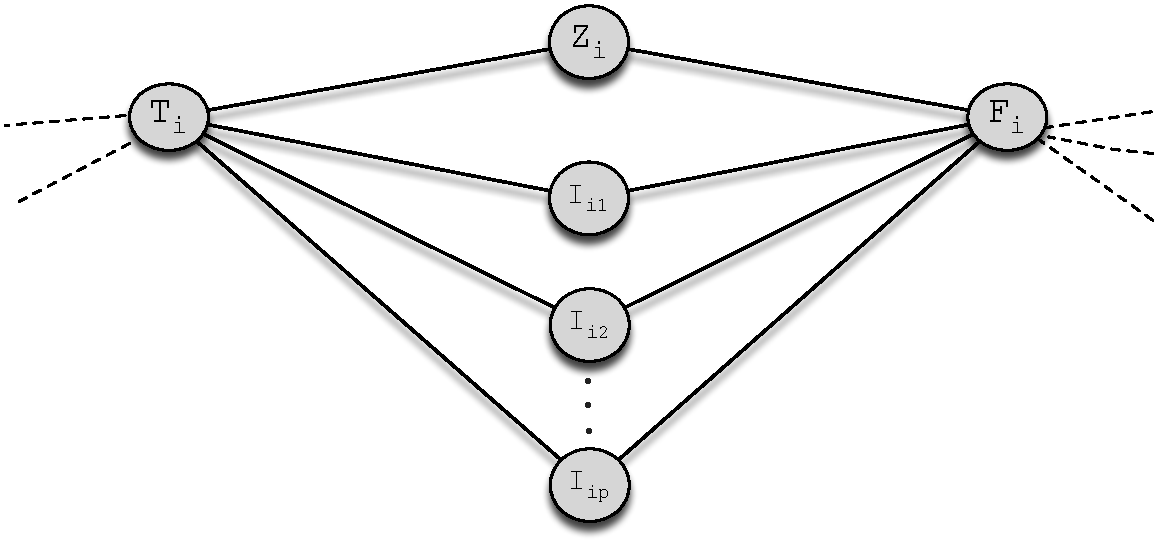
\includegraphics[scale=0.61]{figs/extensions/vgadget-inject-extend.pdf}}
    \subfigure[Modified variable gadget used in \xval and \xvalparts. Each disconnected subgraph has additional injection nodes: nodes $I_{i1}^t, I_{i2}^t, \dots I_{ip}^t$ are added to the upper subgraph
	and nodes $I_{i1}^b, I_{i2}^b, \dots I_{ip}^b$ are included in the bottom subgraph.]
	 {\label{fig:variable-inject-extend2}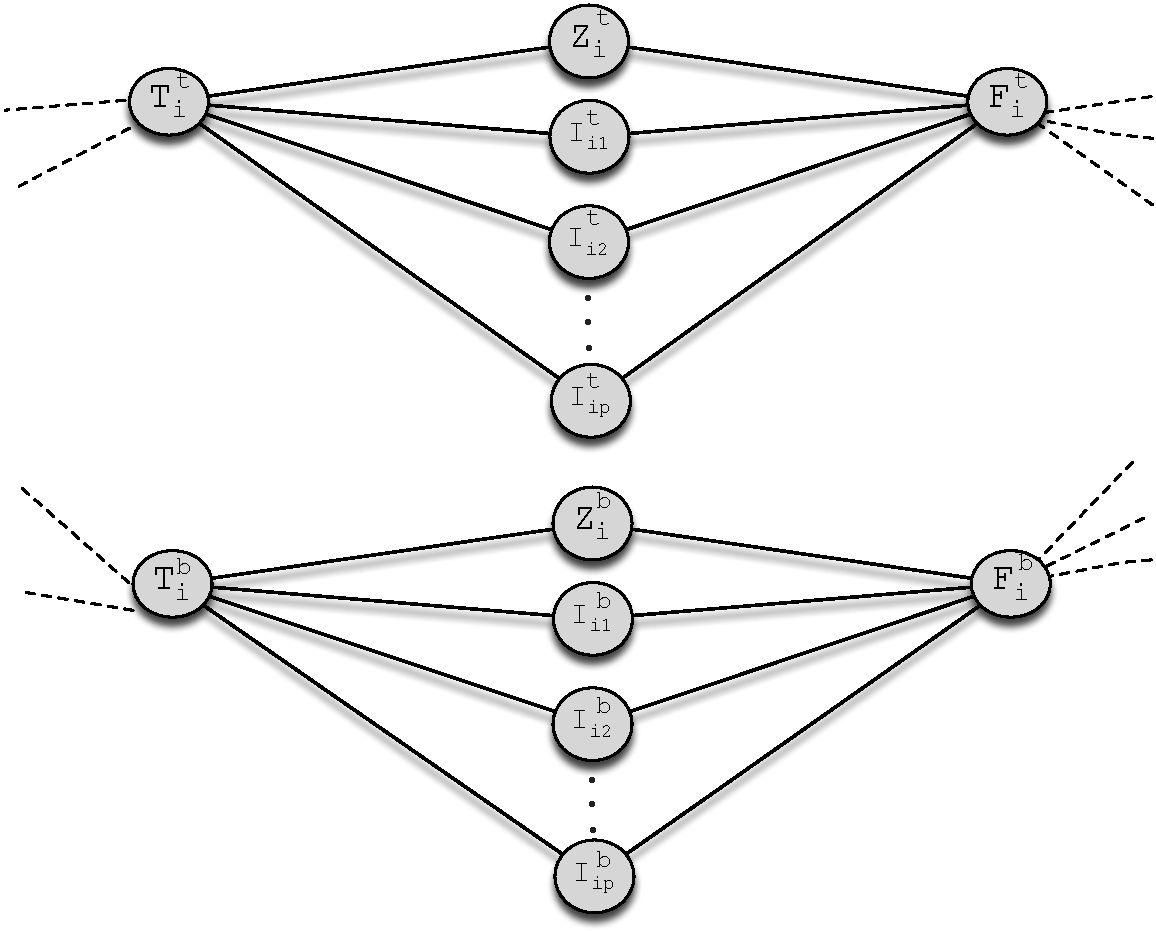
\includegraphics[scale=0.61]{figs/extensions/vgadget-inject-extend2.pdf}}
  \end{center}
	\caption{Figures for variable gadget extensions to include more injection nodes described in Section \ref{subsec:extend}. The dashed edges indicate connections to clause gadget nodes. }
\end{figure}

\begin{figure}
  \begin{center}
    \subfigure[Modified variable gadget used in \full and \maxincs, containing additional injection nodes: $Z_{i1}, Z_{i2}, \dots Z_{ip}$. ]{\label{fig:variable-noninject-extend}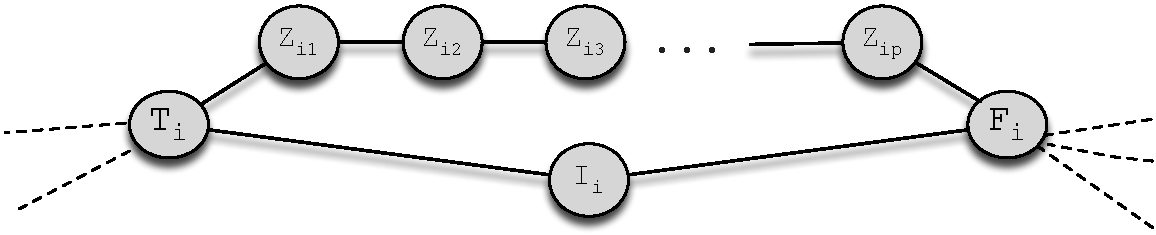
\includegraphics[scale=0.61]{figs/extensions/vgadget-noninject-extend.pdf}}
    \subfigure[Modified variable gadget used in \xval and \xvalparts. Each disconnected subgraph has additional injection nodes: the upper subgraph includes nodes $Z_{i1}^t, Z_{i2}^t, \dots Z_{ip}^t$
	 and nodes  $Z_{i1}^b, Z_{i2}^b, \dots Z_{ip}^b$ are added in the bottom subgraph.]
	 {\label{fig:variable-noninject-extend2}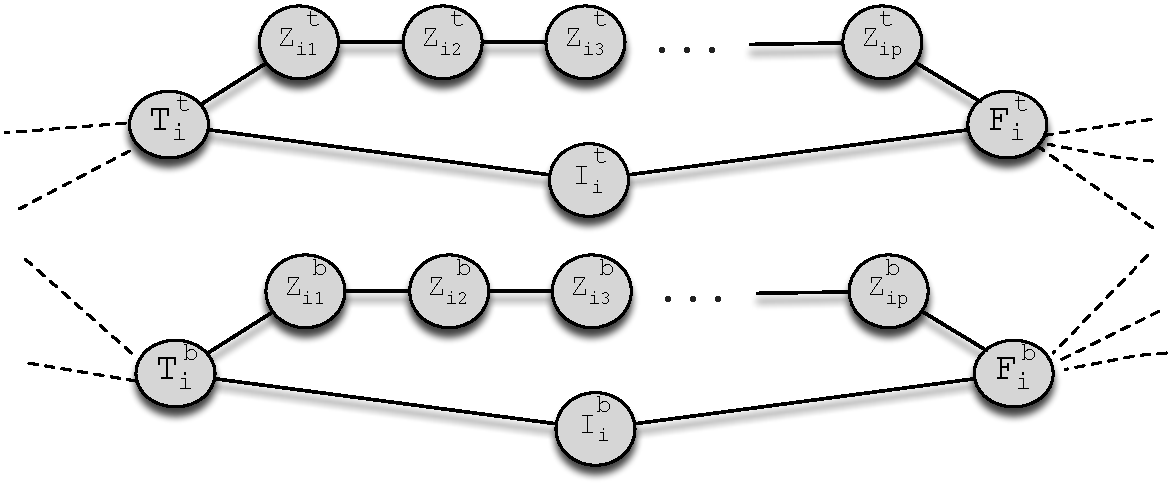
\includegraphics[scale=0.61]{figs/extensions/vgadget-noninject-extend2.pdf}}
  \end{center}
	\caption{Figures for variable gadget extensions to include more non-injection nodes described in Section \ref{subsec:extend}. The dashed edges indicate connections to clause gadget nodes. }
\end{figure}



\begin{figure}
\centering
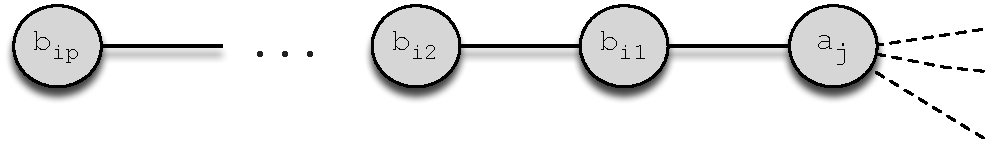
\includegraphics[scale=0.61]{figs/extensions/line-gadget-extend.pdf}
%\includegraphics[scale=0.51]{figs/example2.pdf}
\caption{Extended clause gadget, $C_j'$, used in Section \ref{subsec:extend}. All nodes are injection nodes.}
\label{fig:clause-extend}
\end{figure}


